\documentclass[english]{article}

% Packages
\usepackage[bookmarks]{hyperref}
\hypersetup{
colorlinks,
citecolor=black,
filecolor=black,
linkcolor=black,
urlcolor=black
}
% \usepackage[T1]{fontenc}
% \usepackage[latin1]{inputenc}
\usepackage{amsmath}
\usepackage{amssymb}
\usepackage{amsthm}
\usepackage{enumerate}
% \usepackage{graphicx}

% Definitions
\def\qqq{\mathbb{Q}}
\def\rrr{\mathbb{R}}
\def\zzz{\mathbb{Z}}
\def\zzzp{\mathbb{Z}_p}
\def\zzzn{\mathbb{Z}_N}
\def\zg{\mathbb{Z}_g}
\def\nnn{\mathbb{N}}
\def\xn{\{x_n\}}
\def\yn{\{y_n\}}
\def\zn{\{z_n\}}
\def\an{\{a_n\}}
% \def\qed{$\Box$}
% \newcounter{padic}
\newcounter{examples}
\theoremstyle{plain}
\newtheorem{theorem}{Theorem}[section]
\newtheorem{corollary}{Corollary}[section]
\newtheorem{lemma}{Lemma}[section]
\newtheorem{proposition}{Proposition}[section]

\theoremstyle{definition}
\newtheorem{definition}{Definition}[section]
\newtheorem{example}[examples]{Example}

\theoremstyle{remark}
\newtheorem{remark}{Remark}[section]
%\includeonly{fcsr}
\begin{document}
\title{On Algebraic Shift Registers}
\author{MIDN 1/C Charles Celerier}

\maketitle

\begin{abstract}
  A stream cipher uses pseudorandom sequences to mimic the security of a
  one-time pad. This paper will investigate how bent functions can be used
  to generate lexicographical bent sequences with large 2-adic valuation.
	Rearrangements of these sequences could be effective for filtering the states
	of feedback with carry shift registers (FCSRs) in stream ciphers. The
	non-linearity of lexicographical bent sequences could provide resistance
  for FCSR-based stream ciphers in register synthesis attacks. In this paper, we
	show that it is possible to compute the 2-adic valuation of a bent
  sequence generated by a Maiorana-McFarland class Boolean function.
\end{abstract}

\section{Introduction}

\par Bytes of data, or short sequences of 1's and 0's, are exchanged between
computer systems all over the planet each day on public channels.
Because gentlemen do read each other's mail, it is necessary to secure the
communication of private data sent over public channels. The solution to this
problem is solved by {\em cryptography}, the designing of systems to secure
data exchanges over public channels.

\par The following example is the same basic communication scenario presented
by Trappe in \cite{trappe-washington_intro-to-crypto}.
Let there be two parties, Alice and Bob, who wish to communicate with one another.
A third party, Eve, is a potential eavesdropper. Alice wants to send a message,
known as the {\em plaintext}, to Bob. To accomplish this without Eve knowing
what the message is before it is received by Bob, Alice must {\em encrypt} her message
by some prearranged method, usually involving an {\em encryption key}, to generate
a related message called {\em ciphertext}. The idea is that the sent ciphertext,
even if it is intercepted by Eve, will be difficult to understand and conceal the
plaintext message. Upon receipt of the ciphertext, Bob will {\em decrypt} the message,
usually involving a {\em decryption key}, similar to the encryption of the message,
and obtain the plaintext message.

\begin{figure}[h!]
	\centering
		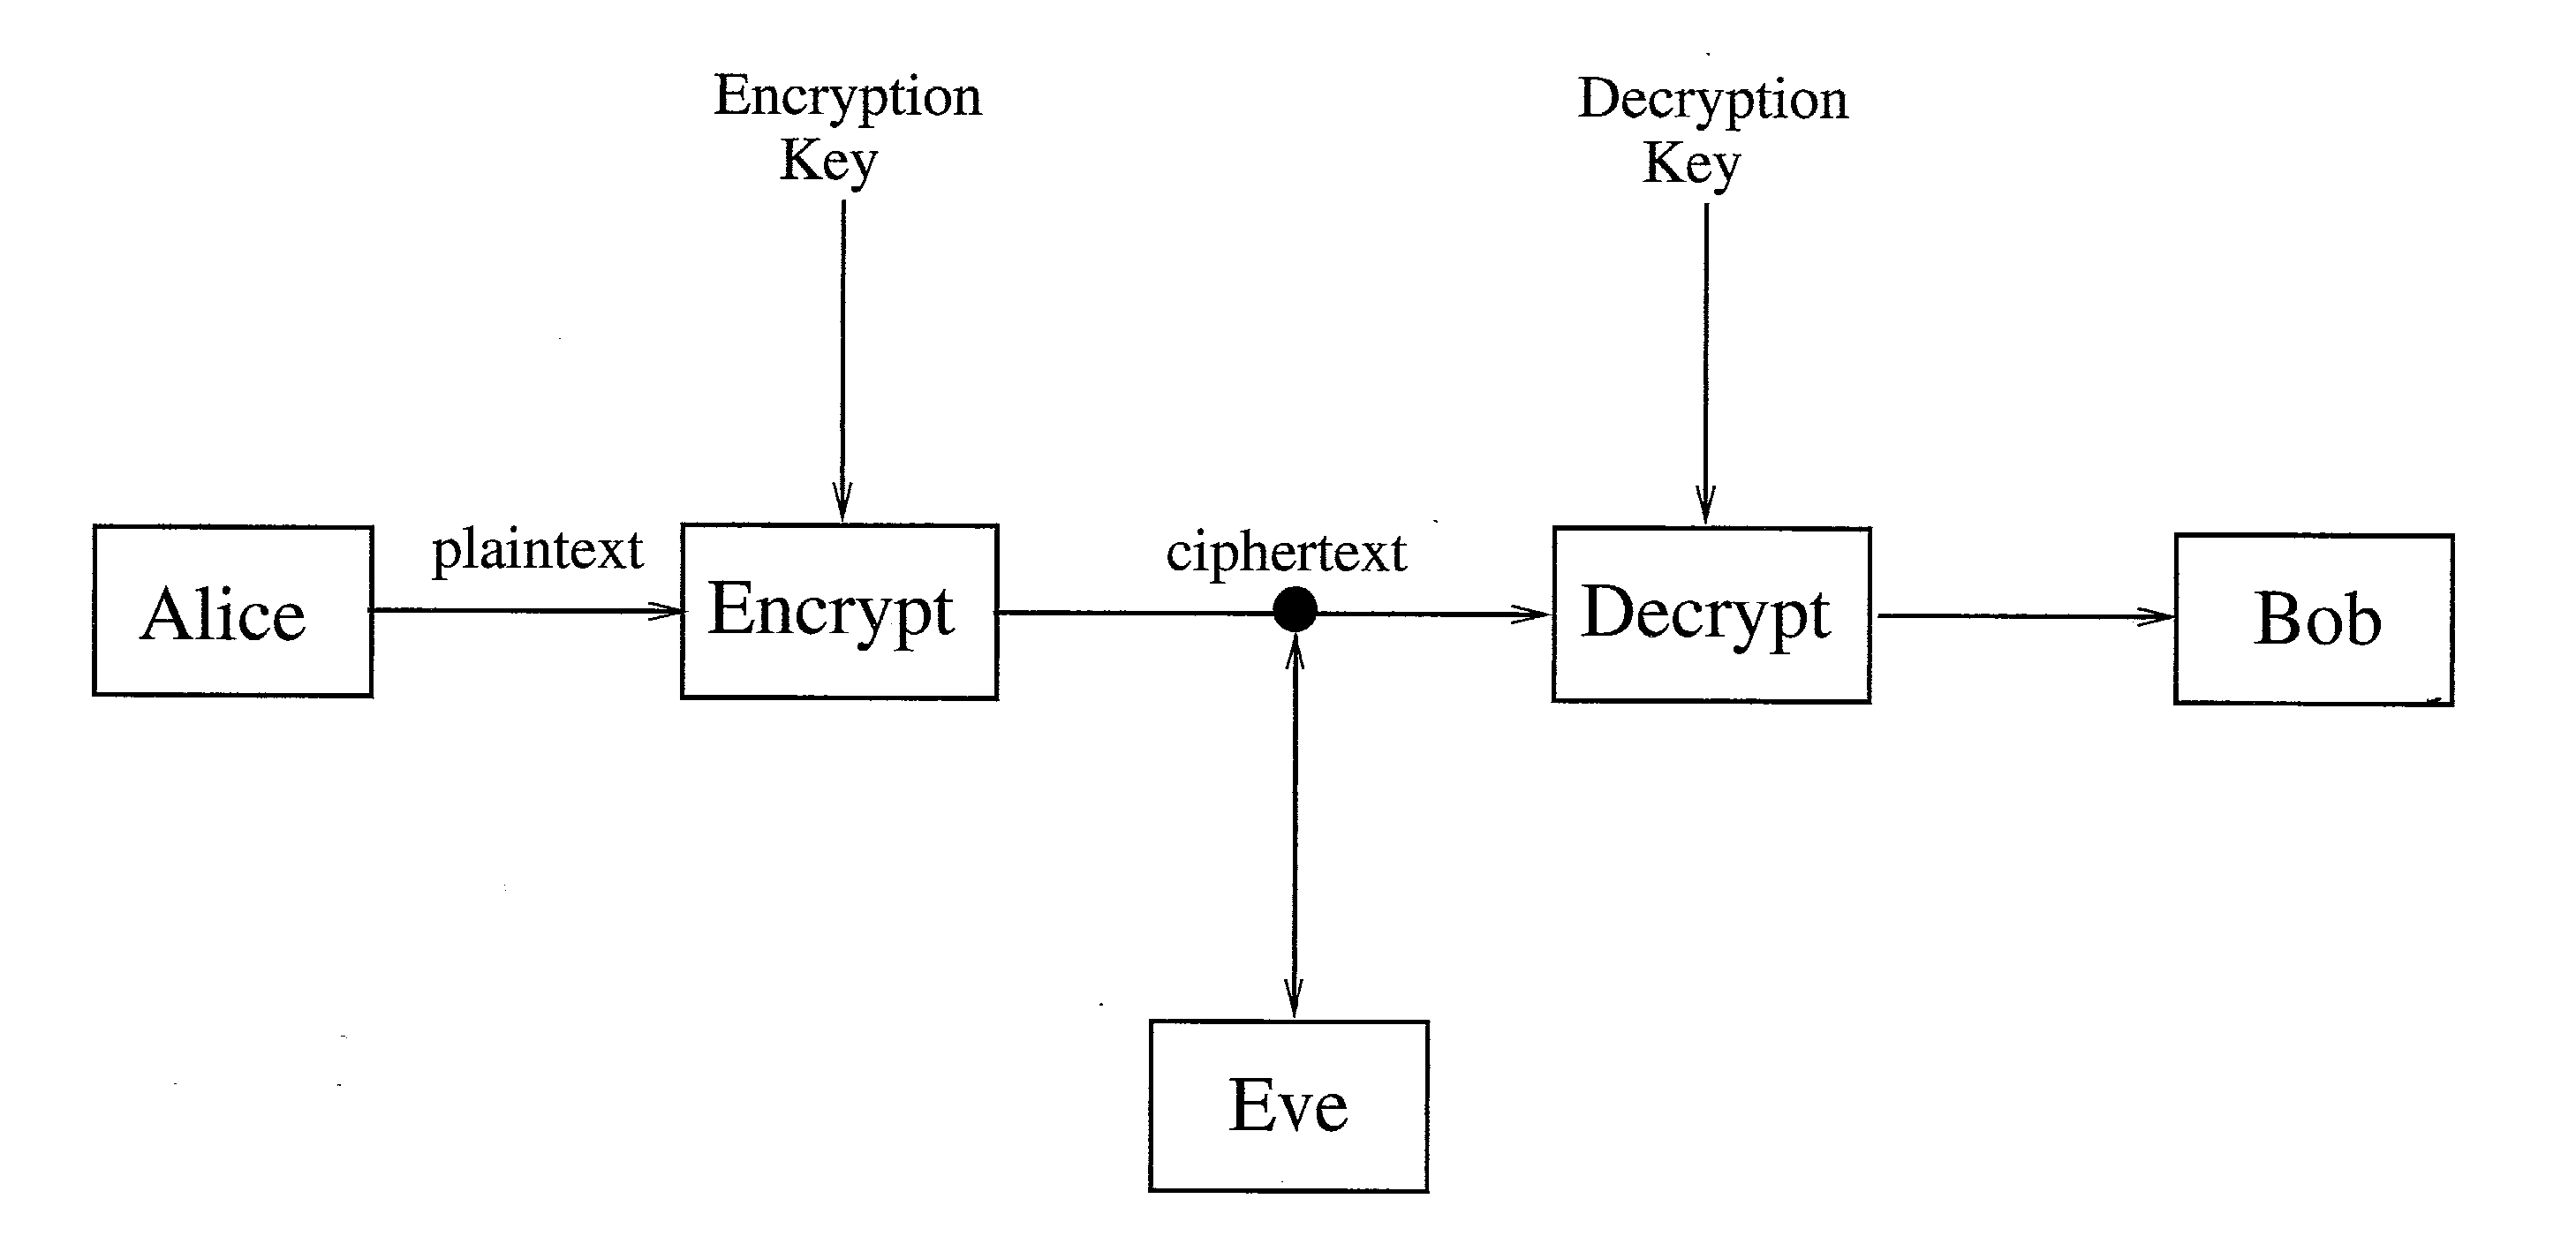
\includegraphics[width=120mm]{figs/basic-scenario.png}
		\caption{The Basic Comunication Scenario for Cryptography \cite{trappe-washington_intro-to-crypto}}
\end{figure}

\par This scenario is the standard example found in many different introductory
cryptography references. Numerous encryption and decryption methods, or {\em cryptosystems},
have been designed to secure the messages sent between Alice and Bob. Unfortunately,
many of these systems have been broken because of the amount of work that goes into
the study of breaking cryptosystems, called {\em cryptanalysis}. A constant battle
exists between the designers and breakers of cryptosystems. In fact, designing
strong cryptosystem typically requires knowledge of cryptography and cryptanalysis.

\par Before diving into the topic of this paper, there is an important assumption that must
be presented. When designing a cryptosystem, every cryptographer assumes {\em Kerckhoffs' principle}:
``In assessing the security of a cryptosystem, one should always assume the enemy knows the method
being used \cite{trappe-washington_intro-to-crypto}.'' The security of a cryptosystem
cannot be based on the concealment of the encryption and decryption algorithms. In practice,
the enemy can obtain the algorithms in many ways, including from the defection or capture
of people. The security must be based on the key and not the algorithm. 

\par Imagine that Alice's message to Bob is a sequence of 1's and 0's, as it would be
in the real world. Consider a cryptosystem which encrypts each bit in the sequence
separately. This would be done by what is called a {\em stream cipher}, which, according to Rueppel,
divides bit sequence into individual bits and enciphers each bit with a time-varying
function whose time-dependency is governed by the internal state of the stream cipher.
The stream cipher can also be thought of in terms of a {\em keystream} which is a
sequence of 1's and 0's the same length of the message that is added to the message
using addition in $\gftwo$ (also known as XOR). If the keystream was perfectly random,
then the cryptosystem would be unbreakable, or {\em perfectly secret}, as
discovered by Claude Shannon in his famous paper ``Communication Theory of Secrecy Systems,''
written in 1945 and published in 1949. This cryptosystem is known as the {\em one-time pad}.
Though it is perfectly secret, it can be difficult to implement because of the inability
to produce perfectly random keystreams. Developing a method to produce perfectly random
sequences is a contradiction in itself. If there is a method to produce the sequence,
then it cannot be perfectly random.

\par Though it is impossible to create perfectly random sequences, it is possible to get close.
This type of sequence is called a {\em pseudorandom sequence}. These sequences have extremely
long periods but are statistically indistinguishable from random sequences. This paper will discuss
the construction of pseudorandom sequences through the use of a particular finite state machine
called the {\em feedback with carry shift register}. It will also investigate the possibility of
incorporating {\em bent functions}, or perfectly non-linear functions, into the construction of
psuedorandom sequences in an attempt to resist synthesizing algorithms. 

\par The paper will follow this basic outline. Important properties of the $p$-adic integers
will be established and examples of different various kinds of $p$-adic integers will be given. 
Then, the finite-state machine will be introduced, followed by the definition of the feedback
with carry shift register. Finally, the boolean functions are defined and described and various
theorems and conjectures will be presented on bent functions.
 
\section{The Ring of $N$-adic Integers}
\par The notation used in the definition of the $N$-adic numbers will follow
the same notation used by Borevich and Shafarevich in Chapter 1 of
{\bf Number Theory}.

\par In this section, the set of $N$-adic integers is shown to be a
commutative ring with an identity.
  
% Definition of N-adic integers
\begin{definition}
\label{def:N-adic}
  Let $N$ be an integer. Then the infinite integer sequence $\xn$
  determines a {\em $N$-adic integer} $\alpha$, or $\xn \rightarrow \alpha$, if
\begin{equation} \label{eq:seq}
  x_{i+1} \equiv x_i \pmod{N^{i+1}} \ \ \ \forall i \geq 0.
\end{equation}
  Two sequences $\xn$ and $\{x_n'\}$ determine the same $N$-adic integer
  if 
\begin{equation} \label{eq:equiv}
  x_i \equiv x_i' \pmod{N^{i+1}}\ \ \ \forall i \geq 0.
\end{equation}
  The {\em set of all $N$-adic integers} will be denoted by $\zzzn$.
\end{definition}

\par Ordinary integers will be called {\em rational integers} and each
rational integer $x$ is associated with a $N$-adic integer, determined
by the sequence \{$x,\ x, \ \dots, \ x,\ \dots$\}.
	
% example of equivalent sequences in Zp
\begin{example} \label{ex:equiv-seq}
  Let $\xn \rightarrow \alpha \in \zzz_3$. Then the first 5 terms of
  $\xn$ may look something like:
  \begin{align*}
    \xn = \{&1 \ , \ 1+2\cdot3 \ , \ 1+2\cdot3+1\cdot3^2 \ , \\
    &1+2\cdot3+1\cdot3^2 \ , \ 1+2\cdot3+1\cdot3^2+1\cdot3^4 \ , \ \dots\} \\
        = \{&1,7,16,16,97,\dots\}
  \end{align*}
  Then equivalent sequences to $\xn$ could begin differently for the
  first few terms:
  \begin{align*}
    \yn &= \{4,25,16,178,583,\dots\} \\
    \zn &= \{-2,-47,232,-308,97,\dots\}
  \end{align*}
  The sequences for $\yn$ and $\zn$ satisfy equation (\ref{eq:seq})
  for the first 5 terms, so they could be $N$-adic integers up to this
  point. Also, both are equivalent to $\xn$ according to the
  equivalence defined in equation (\ref{eq:equiv}).
  \begin{align*}
    &1 \equiv 4 \equiv 2 \pmod 3 \\
    &7 \equiv 25 \equiv -47 \pmod{3^2} \\
    &16 \equiv 16 \equiv 232 \pmod{3^3} \\
    &16 \equiv 178 \equiv -308 \pmod{3^4} \\
    &97 \equiv 583 \equiv 97 \pmod{3^5}
  \end{align*}
  Therefore $\xn,\yn,\zn \rightarrow \alpha$.
\end{example}

\par Because there are infinitely many sequence representations for any $N$-adic
integer, it is useful to define a canonical sequence to be used when
writing $N$-adic integers as sequences.
  
\begin{definition}
\label{def:canon}
  For a given $N$-adic integer $\alpha$, a given sequence $\an$ with
  the properties:
  \begin{enumerate}[i.]
    \item $\an \rightarrow \alpha$
    \item $\an=\{a_0, \ a_0+a_1\cdot N, \ \dots, \ a_0+\dots+a_i\cdot N^i, \ \dots\} : 0 \leq a_i < N \ \ \ \forall i \geq 0$
  \end{enumerate}
  will be called {\em canonical}. The number $a_0a_1a_2 \dots a_i \dots$
  is the {\em digit representation} of $\alpha$.
\end{definition}

% Insert example of a p-adic integer written in canonical form
\begin{example} \label{ex:canon}
  In Example \ref{ex:equiv-seq}, the sequence $\xn$ was a canonical
  sequence that determined the $N$-adic integer $\alpha$. A few more examples
  of canonical sequences determining 7-adic integers are given here:\\
  \\
 $\beta = 3164\dots$, then the canonical sequence $\{b_n\} \rightarrow \beta$ is
  \begin{align*}
    \{b_n\} &= \{3, \ 3+1\cdot7, \ 3+1\cdot7+6\cdot7^2, \ 3+1\cdot7+6\cdot7^2+4\cdot7^3, \ \dots\}\\
            &= \{3,10,304,1676,\dots\}
  \end{align*}
  $\gamma = 0164\dots$, then the canonical sequence $\{c_n\} \rightarrow \gamma$ is
  \begin{align*}
    \{c_n\} &= \{0, \ 1\cdot7, \ 1\cdot7+6\cdot7^2, \ 1\cdot7+6\cdot7^2+4\cdot7^3, \ \dots\}\\
            &= \{0,7,301,1673,\dots\}
  \end{align*}
  $\delta = 5031\dots$, then the canonical sequence $\{d_n\} \rightarrow \delta$ is
  \begin{align*}
    \{d_n\} &= \{5, \ 5, 5+3\cdot7^2, \ 5+3\cdot7^2+1\cdot7^3, \ \dots\}\\
            &= \{5,5,152,495,\dots\}.
  \end{align*}
\end{example}

\begin{definition}
  Addition and multiplication in $\zzzn$ are done term by term. \\
  Let $\alpha,\beta \in \zzzn$ and $\xn \rightarrow \alpha, \yn \rightarrow \beta$. Then,
  \begin{align*}
    \xn+\yn     &:= \{x_0+y_0, x_1+y_1, \dots\} \rightarrow \alpha+\beta\\
    \xn\cdot\yn &:= \{x_0 \cdot y_0, x_1 \cdot y_1, \dots\} \rightarrow \alpha \cdot \beta\\ 
  \end{align*}

  Define $\{0,0,0,\dots\} \rightarrow 0 \in \zzzn$ and $\{1,1,1,\dots\} \rightarrow 1 \in \zzzn$
\end{definition}

\begin{lemma}\label{lem:identity}
  For $\alpha \in \zzzn$, $\alpha+0=0+\alpha=\alpha$ and $1\cdot\alpha=\alpha\cdot1=\alpha$.
\end{lemma}
\begin{proof}
  Let $\xn\rightarrow\alpha\in\zzzn$.
  \begin{align*}
    \xn+\{0,0,\dots\}&=\{x_0+0,x_1+0,\dots,x_i+0,\dots\}\\
                     &=\{x_0,\dots,x_i,\dots\}.\\
    \{0,0,\dots\}+\xn&=\{0+x_0,0+x_1,\dots,0+x_i,\dots\}\\
                     &=\{x_0,\dots,x_i,\dots\}.
  \end{align*}
  $\xn=\xn+\{0,0,\dots\}=\{0,0,\dots\}+\xn$ implies $\alpha=\alpha+0=0+\alpha$.
  Therefore, the additive identity in $\zzzn$ is 0.

  \begin{align*}
    \xn\cdot\{1,1,\dots\}&=\{x_0\cdot 1,x_1\cdot 1,\dots,x_i\cdot 1,\dots\}\\
                         &=\{x_0,\dots,x_i,\dots\}.\\
    \{1,1,\dots\}\cdot\xn&=\{1\cdot x_0,1\cdot x_1,\dots,1\cdot x_i,\dots\}\\
                         &=\{x_0,\dots,x_i,\dots\}.
  \end{align*}
   $\xn=\xn\cdot\{1,1,\dots\}=\{1,1,\dots\}\cdot\xn$ implies $\alpha=\alpha\cdot1=1\cdot\alpha$.
  Therefore, the multiplicative identity in $\zzzn$ is 1.
\end{proof}   
% Insert examples of multiplication and addition

\par Finally, this paper defines a {\em ring} accroding to Fine, Gaglione, and Roesenberger and
shows that $\zzzn$ is a {\em commutative ring with an identity}.
\begin{definition}
\label{def:ring}
{\rm \cite{FGR-Alg-Method}}
  A {\em ring} is a set $R$ with two binary operations defined on it. These are usually
  called addition denoted by +, and multiplication denoted by $\cdot$ or juxtaposition,
  satisfying the following six axioms:
  \begin{enumerate}
    \item Addition is commutative: $a+b=b+a \ \ \forall a,b \in R$.
    \item Addition is associative: $a+(b+c)=(a+b)+c \ \ \forall a,b,c \in R$.
    \item There exists an additive identity, denoted by 0, such that $a+0=a \ \ \forall a \in R$.
    \item $\forall a \in R$ there exists an additive inverse, denoted by $-a$, such
      that $a+(-a)=0$.
    \item Multiplication is associative: $a(bc)=(ab)c \ \forall a,b,c \in R$
    \item Multiplication is left and right distributive over addition:
      \begin{align*}
        a(b+c)&=ab+ac \\
        (b+c)a&=ba+ca
      \end{align*}
      \newcounter{enumi_saved}
      \setcounter{enumi_saved}{\value{enumi}}
  \end{enumerate}
  If it is also true that
  \begin{enumerate}
      \setcounter{enumi}{\value{enumi_saved}}
    \item Multiplication is commutative: $ab=ba \ \ \forall a,b \in R$, then
      $R$ is a {\em commutative ring}.
      \setcounter{enumi_saved}{\value{enumi}}
  \end{enumerate}
  Further if
  \begin{enumerate}
      \setcounter{enumi}{\value{enumi_saved}}
    \item There exists a multiplicative identity denoted by 1 such that
      $a \cdot 1=a$ and $1 \cdot a=a \ \ \forall a \in R$, then $R$ is a
      {\em ring with an identity}.
  \end{enumerate}
  If $R$ satisfies all eight properties, then $R$ is a {\em commutative ring with
  an identity.}
\end{definition}

\begin{theorem}
  $\zzzn$ is a commutative ring with an identity.
\end{theorem}
% p-adic integer ring proof
\begin{proof}
  Let $\xn,\yn,\zn$ determine $\alpha,\beta,\gamma\in\zzzn$ respectively. Then
  \begin{enumerate}
    \item {\em Commutativity of Addition}
      \begin{align*}
            \xn+\yn&=\{x_0+y_0,\dots,x_i+y_i,\dots\} \\
                   &=\{y_0+x_0,\dots,y_i+x_i,\dots\} \\
                   &=\yn+\xn.
      \end{align*}
      $\xn+\yn \rightarrow \alpha+\beta$ and $\xn+\yn=\yn+\xn \rightarrow \beta+\alpha$.
      Therefore, by Definition \ref{def:N-adic}, $\alpha+\beta=\beta+\alpha$.
    \item {\em Associativity of Addition}
      \begin{align*}
        \xn+(\yn+\zn)&=\xn+\{y_0+z_0,\dots,y_i+z_i,\dots\} \\
                     &=\{x_0+(y_0+z_0),\dots,x_i+(y_i+z_i),\dots\} \\
                     &=\{(x_0+y_0)+z_0,\dots,(x_i+y_i)+z_i,\dots\} \\
                     &=\{x_0+y_0,\dots,x_i+y_i,\dots\}+\zn \\
                     &=(\xn+\yn)+\zn.
      \end{align*}
      Therefore, $\alpha+(\beta+\gamma)=(\alpha+\beta)+\gamma$.
    \item {\em Existence of the Additive Identity}
      \\ \\
      By Lemma \ref{lem:identity}, $0$ is the additive identity.
    \item {\em Existence of Additive Inverses}
      \\ \\
      Define $-\xn = \{p-x_0,p^2-x_1,\dots,p^{i+1}-x_i,\dots\} \rightarrow -\alpha$.
      Then
      \begin{align*}
        \xn+(-\xn)&=\{x_0+p-x_0,x_1+p^2-x_1,\dots,x_i+p^{i+1}-x_i,\dots\} \\
                  &=\{p,p^2,\dots,p^{i+1},\dots\} \\
                  &\equiv\{0,0,\dots\} \\
                  &=0.
      \end{align*}
      Therefore, $\alpha+(-\alpha)=0$.
    \item {\em Associativity of Multiplication}
      \begin{align*}
        \xn(\yn\zn)&=\xn\{y_0z_0,\dots,y_iz_i,\dots\} \\
                   &=\{x_0(y_0z_0),\dots,x_i(y_iz_i),\dots\} \\
                   &=\{(x_0y_0)z_0,\dots,(x_iy_i)z_i,\dots\} \\
                   &=\{x_0y_0,\dots,x_iy_i,\dots\}\zn \\
                   &=(\xn\yn)\zn.
      \end{align*}
      Therefore, $\alpha(\beta\gamma)=(\alpha\beta)\gamma$.
    \setcounter{enumi}{6}
    \item {\em Commutativity of Multiplication}
      \begin{align*}
        \xn\yn&=\{x_0y_0,\dots,x_iy_i,\dots\} \\
              &=\{y_0x_0,\dots,y_ix_i,\dots\} \\
              &=\yn\xn.
      \end{align*}
      Therefore, $\alpha\beta=\beta\alpha$.
    \setcounter{enumi}{5}
    \item {\em Left and right distributivity of multiplication over addition}
      \begin{align*}
        \xn(\yn+\zn)&=\xn\{y_0+z_0,\dots,y_i+z_i,\dots\} \\
                    &=\{x_0(y_0+z_0),\dots,x_i(y_i+z_i),\dots\} \\
                    &=\{x_0y_0+x_0z_0,\dots,x_iy_i+x_iz_i,\dots\} \\
                    &=\xn\yn+\xn\zn. \\
      \end{align*}
      By commutativity of multiplication,
      \begin{align*}
        (\yn+\zn)\xn&=\xn(\yn+\zn)\\
                    &=\xn\yn+\xn\zn\\
                    &=\yn\xn+\zn\xn.
      \end{align*}
      Therefore, $\alpha(\beta+\gamma)=\alpha\beta+\alpha\gamma$ and
      $(\beta+\gamma)\alpha=\beta\alpha+\gamma\alpha$.
    \setcounter{enumi}{7}
    \item {\em Existence of a multiplicative identity}
      \\ \\
      By Lemma \ref{lem:identity}, 1 is the multiplicative identity.
      \\ \\
      Properties 1 through 8 from Definition~\ref{def:ring} are satisfied,
      so $\zzzn$ is a commutative ring with an identity.
  \end{enumerate}
\end{proof}

\begin{theorem}\label{thm:units}
  An $N$-adic integer $\alpha$, which is determined by a sequence $\xn$, is
  a unit if and only if $x_0$ is relatively prime to $N$.
\end{theorem}
\begin{proof}
  Let $\alpha$ be a unit. Then there is an $N$-adic integer $\beta$ such that
  $\alpha\beta=1$. If $\beta$ is determined by the sequence $\yn$, then
  \begin{equation}\label{eq:units}
    x_iy_i\equiv1\pmod{N^{i+1}} \ \ \forall i \geq 0.
  \end{equation}
  In particular, $x_0y_0\equiv1\pmod N$ and hence $x_0\not\equiv0\bmod N$.
  Thus, $x_0$ is relatively prime to $N$.
  Conversely, let $x_0$ be relatively prime to $N$. Then $x_0\not\equiv0\pmod{N}$.
  From (\ref{eq:seq})
  \begin{align*}
    x_1 &\equiv x_0 \pmod N\\
    &\vdots \\
    x_{i+1} &\equiv x_i \pmod{N^i}. 
  \end{align*}
  Working backward, $x_{i+1} \equiv x_i \equiv \dots \equiv x_1 \equiv x_0 \pmod N$.
  Thus, $x_i$ is relatively prime to $p \ \ \forall i\geq0$, which implies
  $x_i$ is relatively prime to $N^{i+1}$. Consequently, $\forall i\geq0 \
  \exists y_i$ such that $x_iy_i \equiv 1 \pmod{N^{i+1}}$. Since
  $x_{i+1} \equiv x_i \pmod p^i$ and $x_{i+1}y_{i+1} \equiv x_iy_i \pmod{N^i}$.
  Then, $y_{i+1} \equiv y_i \pmod{N^i}$. Therefore the sequence $\yn$ determines
  some $N$-adic integer $\beta$. Because $x_iy_i \equiv 1 \pmod{N^{i+1}} \ \ \forall i \geq 0$,
  $\alpha\beta=1$. This means $\alpha$ is a unit.
\end{proof}

\par From this theorem it follows that a rational integer $a\in\zzzn$ is a unit if
and only if $a$ is relatively prime to $N$. If this condition holds, then $a^{-1}\in\zzzn$.
Then for any rational integer $b\in\zzzn$, $b/a=a^{-1}b\in\zzzn$.


\section{Constructing Sequences Determing $\frac{b}{a}$ in $\zzzn$}

\par For any rational number $b/a$, $a$ relatively prime to $N$, there
exists a sequence $\xn \rightarrow b/a \in \zzzn$. At this point, it is worth
using the digit representation for integers in $\zzzn$. So
$\xn=\{x_0, \ x_0+x_1N, \ \dots, \ x_0+\dots+x_iN^i, \ \dots\}$
and $b/a = x_0x_1\dots x_i\dots$. Rather than finding $a^{-1}\pmod N^{i+1}$ to
determine each $x_i$, it is not too difficult for every $i$ to find $\sum_{k=0}^ix_kN^k$
such that
\begin{equation}\label{eq:seq-rational}
  b \equiv a\sum_{k=0}^ix_kN^k \pmod{N^{i+1}}.
\end{equation}
Then, 
\begin{equation}
  x_i = \frac{\sum_{k=0}^ix_kN^k - \sum_{k=0}^{i-1}x_kN^k}{N^k}.
\end{equation}

\par Nearly all of the digits for any rational number in $\zzzn$ can also
be found using powers of $N^{-1}$, which is much simpler to analyze
than the brute force search for the digits mentioned above.

\begin{theorem}\label{thm:10}
  Let $u_0,q,N\in\zzz$, where $q$ is relatively prime to $N$,
  $\lvert u_0 \rvert < q$, and $q=-q_0+\sum_{i=1}^{r}q_iN^i$ for
  $0 \leq q_i < N$. Define $\alpha = u_0/q \in \zzzn$
  such that $\alpha = \sum_{i=0}^{\infty}a_iN^i$ for $0 \leq a_i < N$.
  Also, define $u_k\in\zzz$ such that $u_k/q = \sum_{i=k}^{\infty}a_iN^{i-k} \in \zzzn$
  and $\gamma \equiv N^{-1} \pmod q$. Then,
  there exist $u_k$ for every $k\geq0$ such that
  \begin{equation}\label{eq:ak}
    a_k \equiv q^{-1}u_k \pmod N.
  \end{equation}
  If $-q<u_0<0$, then $u_k \in \{-q,\dots,-1\}$ for $k\geq0$.
  Otherwise, for $k>\lfloor \log_N(q) \rfloor=r$, $u_k \in \{-q,\dots,-1\}$
  \\ \\
  Let $\omega \in \{-q,\dots,-1\}$ such that $\omega \equiv \gamma^k u_0 \pmod q$.
  Then for $k>\lfloor \log_N(q) \rfloor=r$, or if $-q<u_0<0$, then $k\geq0$,
  \begin{equation}\label{eq:ak-omega}
    a_k \equiv q^{-1}\omega \pmod N.
  \end{equation}
\end{theorem}
\noindent \\ 
\begin{proof}
%  Let $u_i/q = \sum_{k=i}^{\infty}a_kN^{k-i} \in \zn$. Then,
%  \begin{align*}
%    \frac{u_0}{q} &= a_0+a_1N+a_2N^2+\dots \\ 
%                  &\vdots \\ 
%    \frac{u_i}{q} &= a_i+a_{i+1}N+a_{i+2}N^2+\dots \\
%                  &\vdots
%  \end{align*}
%  It follows that
  Write $u_0/q$ in terms of $u_k$.
  \begin{align}
    \frac{u_0}{q} &= a_0 + N\frac{u_1}{q} = a_0 + a_1N + N^2\frac{u_2}{q} = \dots \nonumber \\
                  &= \sum_{i=0}^{k-1}a_iN^i + N^k\frac{u_k}{q} \ \ \forall k \geq 1. \label{eq:u0/q}
  \end{align}
%  Rewrite (\ref{eq:u0/q}) to be
%  \begin{equation}\label{eq:u0/q-rw}
%    u_0 = q(\sum_{i=0}^{k-1}a_iN^i) + N^ku_k \ \ \forall k \geq 1.
%  \end{equation}
%  For $k=1$, $u_0=qa_0+Nu_1$. Therefore $a_0 \equiv q^{-1}u_0 \pmod N$. This
%  completes half of the theorem.\\
  Rewrite (\ref{eq:u0/q}) to be
  \begin{equation}\label{eq:u0/q-rw}
    p^ku_k=u_0-q\bigg(\sum_{i=0}^{k-1}a_ip^i\bigg) \ \ \forall k \geq 1
  \end{equation}
  Then $\lvert u_0 \rvert < q$ and $0 \leq a_i < p$ from the assumptions
  and equation (\ref{eq:u0/q-rw}). These imply for all $k \geq 1$,
  $\lvert u_0 \rvert = \lvert q\sum_{i=0}^{k-1}a_ip^i + p^ku_k \rvert < q$.
  Then,
  \begin{align*}
    -q-q\sum_{i=0}^{k-1}a_ip^i < p^k&u_k < q-q\sum_{i=0}^{k-1}a_ip^i \\
    \Rightarrow -q\bigg(\frac{1+\sum_{i=0}^{k-1}a_ip^i}{p^k}\bigg) < \ &u_k < q\bigg(\frac{1-\sum_{i=0}^{k-1}a_ip^i}{p^k}\bigg).
  \end{align*}
  $u_k$ may only greater than zero when $\frac{1-\sum_{i=0}^{k-1}a_ip^i}{p^k}$ greater than zero.
  This only occurs when the sequence $[a_0,\dots,a_j] = [0,\dots,0]$ for $j\geq0$.
  Such a sequence occurs if and only if $u_0\geq0$ and $u_0 \equiv 0 \pmod p^i$ for $0\leq i \leq j$, $j\geq0$.
  This is clear from the construction of $p$-adic sequences for
  rational numbers. Therefore $u_k$ may only be greater than zero
  if $u_0\geq0$ and $u_0 \equiv 0 \pmod p^i$ for $0\leq i \leq j$, $j\geq0$.
  The lower bound is greater than $-q$. This clear because
  $\frac{1+\sum_{i=0}^{k-1}a_ip^i}{p^k}\leq1$.
  Therefore,
  \begin{equation*}
    -q < u_k < 0 \ for \ -q<u_0<0.
  \end{equation*}
  If $0\geq u_0<q$, then the upper bound remains unchanged.
  \begin{equation*}
    -q < u_k < q\bigg(\frac{1-\sum_{i=0}^{k-1}a_ip^i}{p^k}\bigg) \ {\rm for} \ 0\leq u_0 < q
  \end{equation*}
  There is still work to be done on the upper bound.
  \begin{align*}
                &0 \leq \sum_{i=0}^{k-1}a_ip^i < p^k \ for \ k\geq1 \\
    \Rightarrow &-q(\sum_{i=0}^{k-1}a_ip^i) \leq 0 \\
    \Rightarrow \ &u_0-q(\sum_{i=0}^{k-1}a_ip^i)<q \\
    \Rightarrow \ &p^ku_k<q \\
    \Rightarrow \ &u_k<\frac{q}{p^k}.
  \end{align*}
  For $k>\lfloor\log_p(q)\rfloor=r$, $\lvert q/p^k \rvert < 1$. Therefore,
  $-q < u_k < 0 \ {\rm for} \ 0\leq u_0 < q \ {\rm and} \ k>r$.
  Further lowering the upperbound, if $u_k=0$, then $u_0/q=\sum_{i=0}^{k-1}a_ip^i+0$.
  This implies $u_0/q$ is a rational integer, which is not true. Noting finally
  that $u_k$ must be an integer. If $\lvert u_0 \rvert<q$ and $u_0<0$, or
  $\lvert u_0 \rvert<q$, $u_0\geq0$, and $k>\lfloor \log_p(q) \rfloor=r$, then
  \begin{equation*}
    u_k \in \{-q,\dots,-1\}.
  \end{equation*}
  It has now been shown for certain restrictions $u_k$ belongs to a specific
  set of representatives for the residue classes of $\zzz/(q)$. Define 
  $\gamma \equiv p^{-1} \pmod q$. Reducing (\ref{eq:u0/q-rw}) modulo $q$ shows that
  \begin{equation}
    u_k \equiv \gamma u_{k-1} \pmod q.
  \end{equation}
  Since this is true for all k greater than or equal to 1, it is clear that
  \begin{equation}\label{eq:uk-mod-q}
    u_k \equiv \gamma^ku_0 \pmod q.
  \end{equation}
  Reducing (\ref{eq:u0/q-rw}) modulo $p$ shows that
  \begin{equation}\label{eq:ak-mod-p}
    a_k \equiv q^{-1}u_k \pmod p.
  \end{equation}
  Define $\omega \equiv \gamma^k u_0 \pmod q$, and $\rho \equiv q^{-1} \bmod p$.
  Finally, if $\lvert u_0 \rvert<q$ and $u_0<0$, or
  $\lvert u_0 \rvert<q$, $u_0\geq0$, and $k>\lfloor \log_p(q) \rfloor=r$, then
  \begin{equation}\label{eq:ak-done}
    a_k \equiv \rho\omega \pmod p.
  \end{equation}
\end{proof}
\begin{corollary}\label{cor:aj}
  Let $0\leq u_0 < q$. Define $j$ to be the greatest integer such that
  $u_0 \equiv 0 \pmod p^j$. Then the following are true:
  \begin{enumerate}[i.]
    \item $j\leq\lfloor\log_p{q}\rfloor = r$
    \item $[a_0,\dots,a_{j-1}]=[0,\dots,0]$
    \item $u_k>0$ for $k=j$
    \item $u_k \not\equiv 0 \pmod p$
  \end{enumerate}
\end{corollary}
\par The results of this corollary are straightforward.

\par Theorem \ref{thm:10} shows that for $-q<u_0<0$, there is a sequence of
numerators $\{u_k\}$ directly related to the sequence of digits $\{a_k\}$
for $u_0/q\in\zn$. This is provides a more powerful tool for the analysis
of the sequences generated by AFSRs. The results shown here fill in the gaps of
the incorrect proof shown in Theorem 10 of Klapper and Xu's paper.


\section{The $p$-adic Metric and Completeness}
  To prove completeness of the set of $p$-adic, we will begin
  by introducing a valuation function. From this point we will
  define the $p$-adic metric and concluding with a proof showing
  that $\zzzp$ satisfies the Cauchy criterion.

\label{pval}
\begin{definition}
  Let $\alpha=\an\in\zzzp\setminus\{0\}$. If $m$ is the smallest
  number in $\nnn$ such that $x_m \not\equiv 0 \pmod p^{m+1}$,
	then the {\em valuation} of $\alpha$ is $m$, or $v_p(\alpha)=m$. \\ \\
  
  If $\alpha=0$, then $v_p(\alpha)=\infty$.
\end{definition}

\label{pnorm}
\begin{definition}
	If $\alpha \in \zzzp$, then the {\em $p$-adic norm} of $\alpha$ is
  $\lVert \alpha \rVert_p = p^{-m}$ where $m = v_p(\alpha)$. 
\end{definition}

% \begin{definition}
% Given a sequence of $p$-adic integers $\{\alpha_n\}$. The sequence is bounded by an integer $M$ if
% \[
%   \lVert \alpha \rVert_p \leq p^{-M} \ \ \ \forall \alpha_i \in \{\alpha_n\}. 
% \].
% \end{definition}
%
% \begin{theorem}
% For every sequence of $p$-adic integers there exists a convergent subsequence.
% \end{theorem}
% 
% \begin{proof}
% Let $\{\alpha_n\}$ be a sequence of $p$-adic integers. Then
% \[
%  \lVert \alpha_i \rVert_p \leq p^0 = 1 \ \ \ \forall i \in \nnn.
% \]
% Define
% \[
%   \alpha_i=\{a_{0,i},a_{0,i}+a_{1,i}*p,a_{0,i}+a_{1,i}*p+a_{2,i}*p^2,...\} \ \ \ \rm{for} \ 0 \leq a_{j,k} < p 
% \]
% \end{proof}

\begin{definition} \label{def:cauchy}
	A sequence $\{\alpha_n\}$, where $\alpha_i\in\zzzp$, {\em converges}
  if \ $\exists\alpha\in\zzzp \ s.t. \\ \forall \ \epsilon>0 \ 
  \exists N \in\nnn \ s.t. \ \forall \ n \geq N \Rightarrow \lVert\alpha_n-\alpha\rVert_p<\epsilon \ .$
\end{definition}

\section{Feedback with Carry Shift Registers}
\par A description of algebraic feedback shift registers specific to $\zzzp$ is defined here.
The definition of the register follows the one given in Andrew Klapper's book.

\begin{definition}\label{afsr}
  Let $q_0,q_1,\dots,q_m\in\zzz/(p)$ for $p\in\zzz$ and assume that $q_0\not\equiv0\pmod p$.
  An {\em algebraic feedback shift register} (or {\em AFSR}) over ($\zzz$,$p$,$S$) of length m with
  {\em multipliers} or {\em taps} $q_0,q_1,\dots,q_m$ is a discrete state machine whose states are
  collections
  \[
  (a_0,a_1,\dots,a_{m-1};z) \ where \ a_i\in S \ and \ z \in \zzz
  \]
  consisting of cell contents $a_i$ and memory $z$. The state changes according to the
  following rules:
  \begin{enumerate}[1.]
    \item Compute
      \[
      \sigma = \sum^m_{i=1}q_ia_{m-i}+z.
      \]
    \item Find $a_m\in S$ such that $-q_0a_m\equiv\sigma\pmod p$. That is $a_m\equiv-q_{0}^{-1}\sigma\pmod p$.
    \item Replace $(a_0,\dots,a_{m-1})$ by $(a_1,\dots,a_m)$ and replace $z$ by $\sigma({\rm div} p) = (\sigma+q_0a_m)/p$.
  \end{enumerate}
\end{definition}

\section{Xu's Rational Approximation Algorithm}
\par In Andrew Klapper's book, he roughly describes Xu's rational approximation
algorithm for $\pi$-adic sequences in any ring $R$. A description of Xu's Algorithm
is presented here in the context of the ring $\zzzp$, where $p$ does not have to be prime.

\par The rational approximation problem is presented here: Given the eventually
periodic digit representation of $frac{a}{b}\in\zzzp$, find $a$ and $b$.

\par If there are no constraints on $a$ and $b$, then the entire sequence must be known
to solve the problem. Specifically, a single algebraic feedback shift register can
not produce all $frac{a}{b}\in\zzzp$.


\bibliographystyle{amsplain}
\bibliography{refs}
\end{document}
